\section{Methodology}

\subsection{Architecture}

\begin{figure}[h]
    \centering
      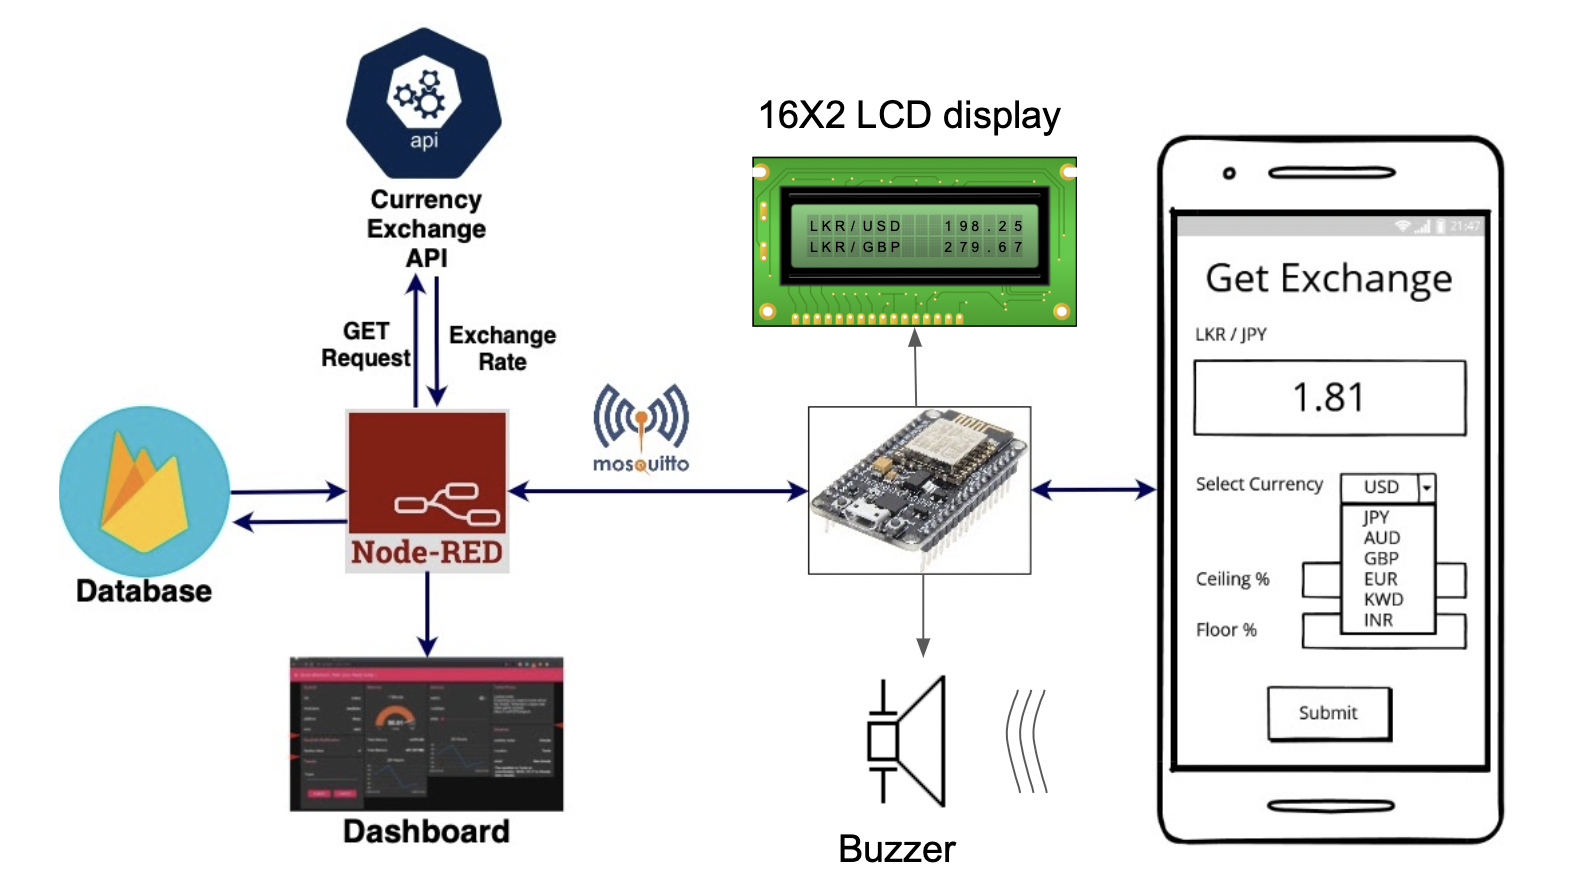
\includegraphics[width=1\textwidth]{images/arch.png}
    \caption{Architecture of the entire solution}
    \label{fig:arch}
\end{figure}

The login credentials of the users of this application are entered to the database from the backend by the database administrator. The user is able to log  in to the application using his/her mobile phone via a website hosted on a NodeMCU. The log in credentials are communicated to a Node-RED application via an MQTT broker and validated with the credentials stored in the Firebase database. On successful authentication, the Node-RED would publish a Success message token to admit the user.\\

Next, the user has the ability to select a currency of preference and specify the ceiling and floor thresholds. These values will also be communicated to the Node-RED application through a MQTT topic, and stored in the Firebase database.\\

A timer which is sending API requests at hourly intervals extracts the currency exchange rates and stores it in the database. The proposed architecture for this project requires exchange rate data every 30 seconds to accurately capture the minor changes in exchange rates, but the free version of the API only provides hourly exchange rate prices. We store these hourly exchange rates in the firebase database and use a gaussian random number generator to vary the hourly exchange rates by minor values to simulate rapid fluctuations of exchange rates similar to their real variations. The ceiling and floor values are checked against these simulated exchange rates at 30 second intervals, and if they are exceeded, an email is sent to the user. The exceeded message is sent to the NodeMCU via the MQTT broker and the Buzzer is sounded as well. This notifies the user in case he/she is offline.\\

The hourly exchange rate data is then used by the Node-RED application to calculate the following four technical indicators.\\

\begin{enumerate}[itemsep=-1.7mm]
\item Simple Moving Average (SMA)
\item Rate of Change oscillator (ROC)
\item Moving average convergence/divergence (MACD)
\item Relative Strength Index (RSI)
\end{enumerate}

These indicators calculated using exchange rate data over 40 hours are plotted on a live dashboard. 

\subsection{Functionalities of NodeMCU}

\begin{figure}[h]
    \centering
      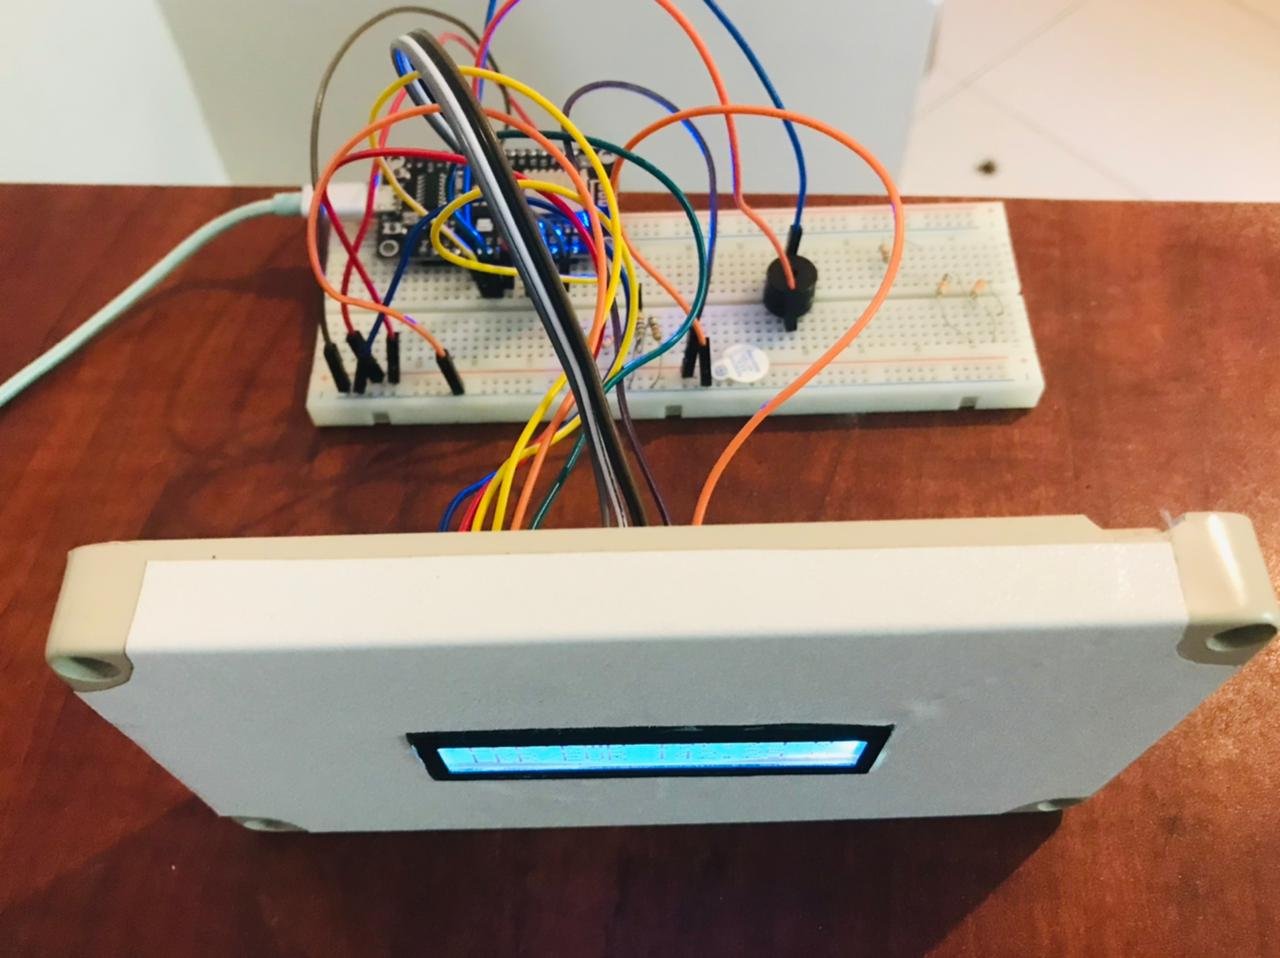
\includegraphics[width=0.7\textwidth]{images/front.png}
    \caption{Setting up ESP8266 with an LCD display and a buzzer}
    \label{fig:front}
\end{figure}

The NodeMCU used in the IOT system performs multiple tasks to facilitate the connectivity between the user’s device, the LCD display, and the buzzer. ESP8266 NodeMCU was used in the testing process. The flow chart in the figure ~\ref{fig:overall}, describes the functionality of the NodeMCU.

\subsubsection{Initial setup}

When the NodeMCU is powered up, it follows a sequence of steps to make sure it is connected to the internet. In order to implement this sequence, 'WiFi manager' library was used.

As the first step,it sets it up in \textit{Station mode} and tries to connect to a previously saved Access Point.

In case it is unsuccessful, NodeMCU will act as an access point with the SSID 'IoT6B\_G05' and create a web server (Default IP \textbf{198.168.4.1}). The user can connect to this access point through any WiFi enabled device and go to the above mentioned IP address using a web browser. The web browser will display the available WiFi access points near the user. By providing the WiFi password of the preferred access point, NodeMCU can connect to the access point. Now the NodeMCU is connected to the internet.

\begin{figure}[H]
    \centering
      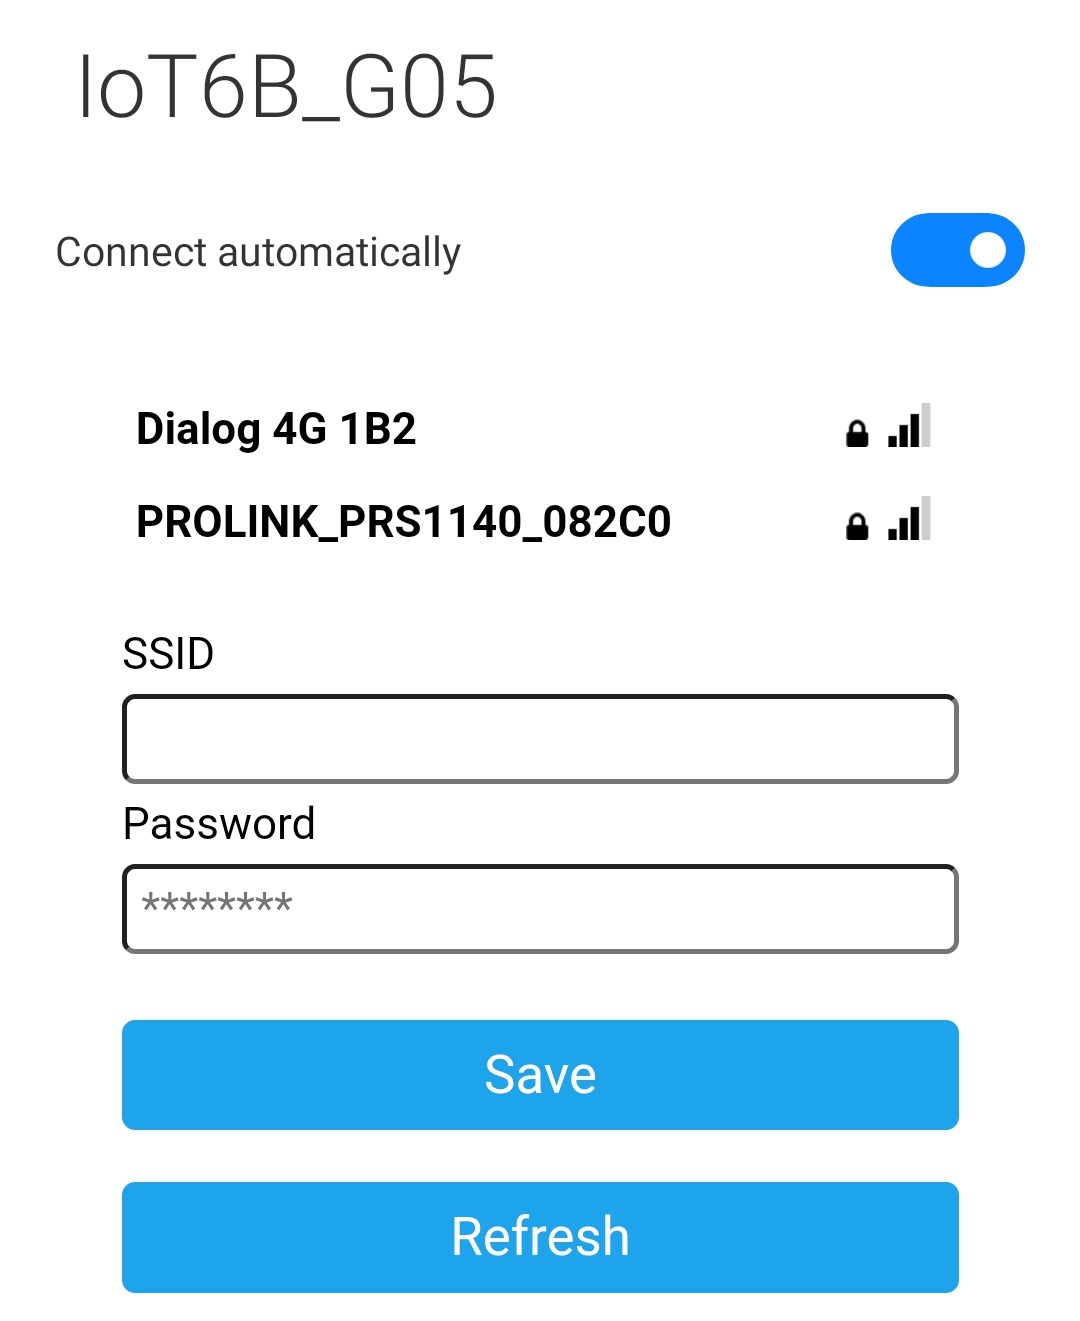
\includegraphics[width=0.4\textwidth]{images/wifilogin.jpeg}
    \caption{WiFi login interface for user}
    \label{fig:wifilogin}
\end{figure}

\subsubsection{Hosting Web Interface for User}

\begin{figure}[H]
    \centering
      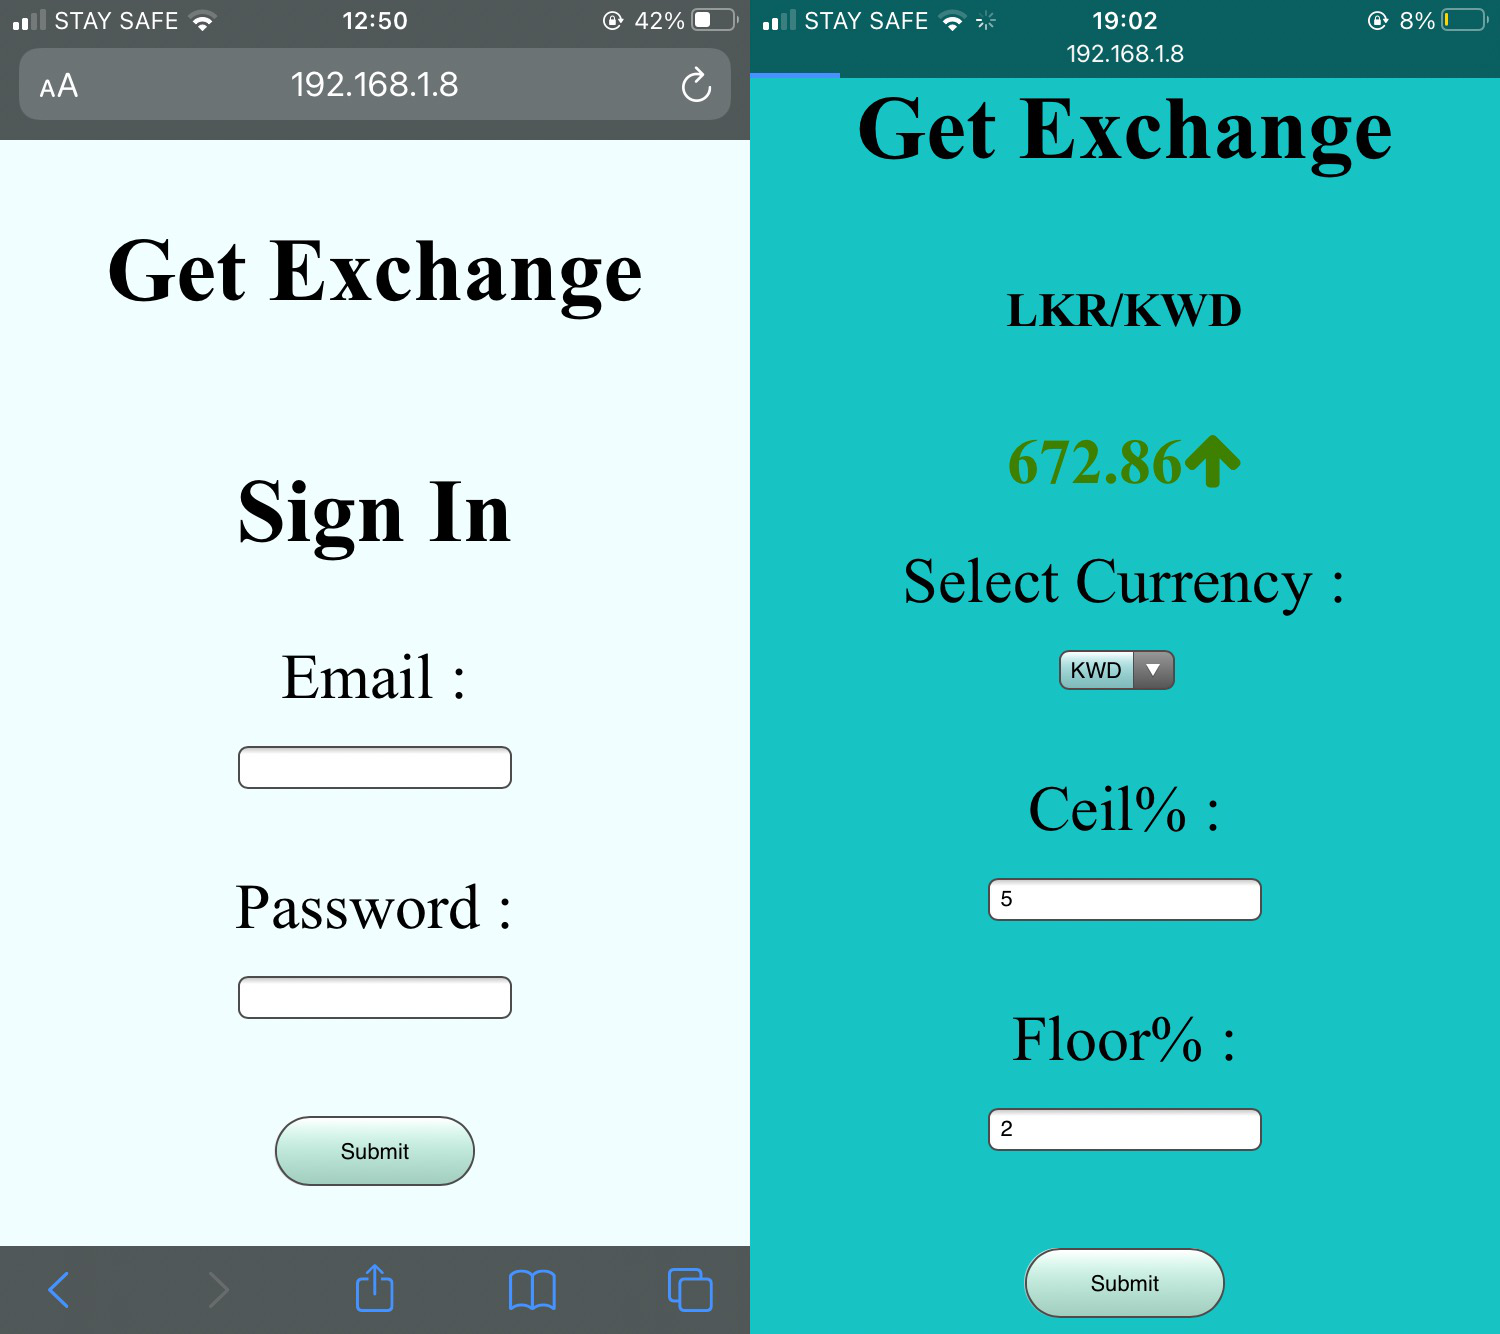
\includegraphics[width=0.7\textwidth]{images/login.png}
    \caption{Login page and home page for the user}
    \label{fig:host}
\end{figure}

The above code calls two functions that return HTML scripts, which enable two HTML pages in figure \ref{fig:host} to be displayed. When the user loads \textbf{192.168.1.8} in the web browser, the login page on the left will appear in the mobile. After the authentication details are submitted, the user is redirected to the home page given that the authentication is successful.\\

In the home page. The user can select a preferred currency out of six available currencies. Additionally, the user can select two percentages to set the ceiling and floor prices compared to the current price. The current price of the selected exchange rate is then displayed on the home page.

\subsubsection{Authentication and authorization flow}

An authentication and an authorization flow is included in the IOT system. This flow is included in figure \ref{fig:overall}. The first step of authentication is the initial login page that requests the user to enter an email and a password. After obtaining the username and the password, NodeMCU sends authentication data to Node-RED through MQTT. Node-RED acts as an authorization server and generates an application access token. This access token is sent back to the NodeMCU through MQTT. NodeMCU then stores the access token along with the user name. Whenever NodeMCU is sending user specific data to Node-RED, the access token is also sent along with it to verify the validity of the user.

\subsubsection{Setting up the MQTT Broker}

The Mosquitto MQTT \cite{mosq} server/broker was used to establish communications between the NodeMCU and the Node-RED application.The messages were published and received in the string data type and each component of the message was separated by a “\$” sign for encoding. This allows several types of information to be transmitted using a single message.\\

The NodeMCU subscribes to four MQTT topics (a., b., c., and d. below), and publishes to two MQTT topics (d., and e.).\\

\textbf{a. IOT\_6B/G05/UserAuth}\\

The login credentials of the user are sent to the Node-RED application for validation through this topic. The format of the published message is as follows.


\begin{center}

\includegraphics[width=0.7\textwidth]{images/userauth.pdf}
\end{center}


\textbf{b. IOT\_6B/G05/AuthResponse}\\

The Nod-RED publishes the response status of the user authentication to this topic and is received by the NodeMCU. The format of the published message is as follows.

\begin{center}
      
\includegraphics[width=0.7\textwidth]{images/authres.pdf}
\end{center}

\textbf{c. IOT\_6B/G05/UserNeeds}\\

The Nod MCU publishes the currency type subscribed to by a particular user, along with the ceiling and floor values requested for notifications. The format of the published message is as follows.


\begin{center}
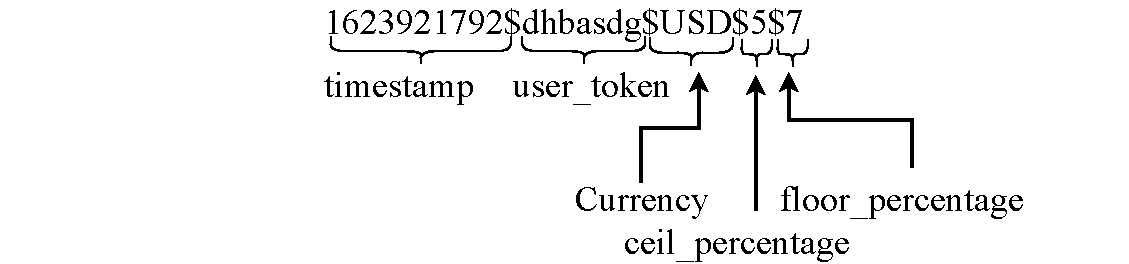
\includegraphics[width=0.7\textwidth]{images/userneeds.pdf}
\end{center}


\textbf{d. IOT\_6B/G05/UserNeedsResponse}\\

The response token from the Node-RED, stating the validity of the request message sent to the IOT\_6B/G05/UserNeeds topic, is published to this topic.  The format of the published message is as follows.


\begin{center}

\includegraphics[width=0.7\textwidth]{images/userneedsres.pdf}
\end{center}


\textbf{e. IOT\_6B/G05/CommonData} \\

This topic  receives the exchange rates of all 6 currency types and is updated every 30 seconds from the Node-RED. These values are received by the NodeMCU, and displayed on the LCD screen. The exchange rate of the selected currency type is displayed on the web interface for the user. The format of the published message is as follows.

\begin{center}
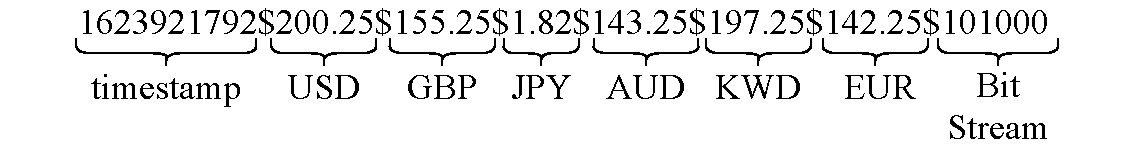
\includegraphics[width=0.7\textwidth]{images/commondata.pdf}
\end{center}

\textbf{f. IOT\_6B/G05/BuzzerNotification} \\

Messages are published to this topic by the Node-RED application when the ceiling and floor prices, specified by the user, have been exceeded by the exchange rate. The format of the published message is as follows.

\begin{center}
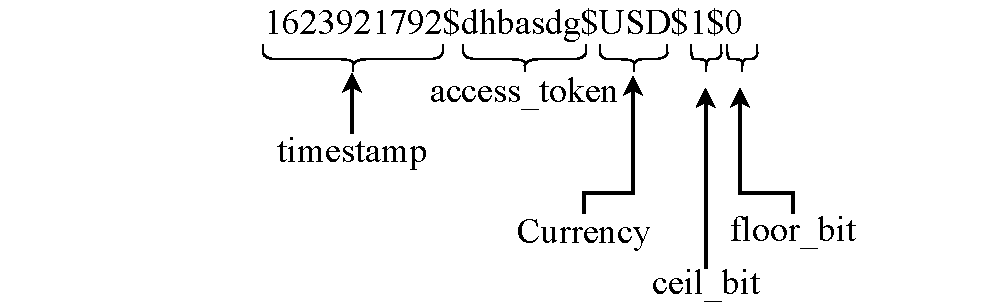
\includegraphics[width=0.7\textwidth]{images/buzzernot.pdf}
\end{center}

The components of the encoded MQTT messages are as follows.

\begin{itemize}[itemsep=-1.7mm]

\item \textbf{timestamp} - Time at which the data is sent in Unix epoch format. This helps to validate timely data and to discard older messages.
\item \textbf{ceil\_bit} - A flag bit which is set to 1 if the ceiling price is crossed, else zero
\item \textbf{floor\_bit} - A flag bit which is set to 1 if the floor price is crossed, else zero
\item \textbf{Bit stream} - Each of the 6 bits corresponds to the 6 currency types and is set to 1 if there is an increase in the exchange rate, 0 otherwise.
\item \textbf{access\_token} - Indicates that the application is authorized to access user’s data \cite{token}

\end{itemize}


MQTT transmissions occur at random times, and the inclusion of the timestamp in the messages facilitated them to be checked to identify old messages. Those which took more than 20 seconds for transmission are discarded. Combining the data using this encoding scheme was required, because several components of the data are used at a certain instance. Further, this method of encoding and transmitting data allowed the LCD display to be updated in one transmission.\\

This simple encoding scheme allows more data to be transmitted with little overhead which can help reduce the power usage of the NodeMCU.

\newpage

\begin{figure}[H]
    \centering
      \includegraphics[width=1\textwidth]{images/overallmin.png}
    \caption{Complete technical process flow chart of the Methodology}
    \label{fig:overall}
\end{figure}

\newpage

\subsubsection{Decoding compact received data}

The goal here is to decode this large string containing several information components, separated using “\$” signs and to assign each of them to separate variables in the NodeMCU, as shown below. \\


1623921792\$200.25\$155.25\$1.82\$143.25\$197.25\$142.25\$101000\\


timestamp = 1623921792, USD = 200.25 , GBP = 155.25, JPY = 1.82, AUD = 143.25, KWD = 197.25 , EUR = 142.25\\

When a subscribed topic receives a data item, the \textbf{callback} function is called. The function considers the topic from which data is received and directs the data to the relevant purpose. For example, the \textbf{process\_notification}  function takes data from the \textbf{“IOT\_6B/G05/BuzzerNotification”} topic, \textbf{process\_Data} function takes data from the \textbf{“IOT\_6B/G05/CommonData”}, etc. An extract of the \textbf{callback} function is given below.\\

\begin{lstlisting}[language=C++]
void callback(char* topic, byte* payload, unsigned int length) {
  if (String(topic) == "IOT_6B/G05/BuzzerNotification") {
   process_notification(payload, length, 50, 5);
  }
  if (String(topic) == "IOT_6B/G05/CommonData") {
   process_data(payload, length, 70, 8);
  }
	:
	:
}
\end{lstlisting}

\vspace{\baselineskip}
The \textbf{process\_notification} function given below, splits the byte array into character arrays and then saves them in the variables treating them as separate cases, at every \textbf{callback} call.\\

\begin{lstlisting}[language=C++]
void process_notification(byte* payload, unsigned int length, int charlen, int numitem) {

     int digit;
     payloadstr = "";
     Serial.println();
     for (int i = 0; i < length; i++) {
       payloadstr += (char)payload[i];
     }

     char payloadstr_array[charlen];
     payloadstr.toCharArray(payloadstr_array, charlen);

     char * token = strtok(payloadstr_array, "$");
   
     for (int i = 1; i < numitem+1; i++) {
        switch (i) {
         case 1:
            timestamp = atol(token);
            Serial.print(timestamp);
            Serial.println();
            break;
	:
	:
         }
         token = strtok(NULL, "$");
     }
}
\end{lstlisting}

\subsubsection{Sensing alerts and notifying the user}

When an alert is sent through the \textbf{“IOT\_6B/G05/BuzzerNotification”} topic, the callback function instantly identifies a crossing in ceiling or floor prices, if any, and activates the \textbf{buzzer}. 
To identify notifications which have expired is essential, to ensure that the user is alerted based on timely information only. The NodeMCU was configured to be updated with the time and date so that it could be compared with the timestamp of received notification messages in unix epoch time format. A sample code is given below.\\

\begin{lstlisting}[language=C++]
if (timestamp > unix_epoch - 19820) {
    current_user = String(token);
}
\end{lstlisting}

\subsubsection{Supporting the LCD 16x2 display}

\begin{figure}[H]
    \centering
      \includegraphics[width=0.4\textwidth]{images/lcd.png}
    \caption{LCD display showing currency values time and date}
    \label{fig:lcd}
\end{figure}


LCD display is used to show the live currency prices updated every 30 seconds, along with the date and time. These values are displayed one after the other, each being displayed for 2 seconds. The time and date was obtained using an available library (the NTPClient library) for NodeMCU, which enables it to communicate with an NTP (Network Time Protocol) Server.\\

\subsubsection{Power Saving Mechanisms of the NodeMCU}

The NodeMCU, along with the LCD display and the buzzer are power constrained devices. Hence power saving methods must be implemented to improve energy efficiency.\\

The main power saving method is by implementing the sleep function in the NodeMCU. When the Foreign exchange markets are closed during the weekends, the Node MCU enters the deep sleep mode to conserve power. Meanwhile, the dashboards from Node-RED are available for the user to monitor the exchange rate fluctuations. However, the maximum NodeMCU deep sleep time is 3 hours and 46 minutes \cite{deepsleep} and if the NodeMCU is kept in deep sleep mode for too long, it may stay in the sleep mode forever. The deep sleep mode is scheduled to begin 15 minutes after the time at which the Forex market is closed and then enters a series of sleep-wake-sleep cycles until 15 minutes before the market is set to open.\\

15 minutes after the market closes, the NodeMCU is set to sleep for an hour. Then it wakes up, and checks whether the market is open or closed using the current time and date. If it is closed, the NodeMCU goes back to sleep for another hour. This is continued till the market opens. NodeMCU is set to keep sleeping every week from Saturday 1.45 a.m. to Monday 2.15 a.m \cite{hours}.\\

The second power saving mechanism used in this application is the use of a simplified message encoding scheme in the form of a string of messages separated by “\$” signs. The same can be done using messages in JSON format, but this would require an additional library to be installed in the ESP8266, as well as a much larger overhead for the messages which are transmitted. The reduction of the message size in the encoding scheme suggested in this project actively reduces the power consumed in data transmission.
